\documentclass[../summary.tex]{subfiles}

\begin{document}
	
	\section{Raw materials and circular economy}
	
	\subsection{Study guide}
	
	Make sure to understand:
	\begin{itemize}
		\setlength{\itemsep}{0pt}
		\item  Meaning of the terms (non-)renewable resources, (in-)finite resources, critical materials
		\item The drivers of material demand (i.e. understand the I-PAT equation and past and predicted evolutions of the constituent factors), including also influence of the energy transition on predicted material demand
		\item Different types of scarcity, including examples
		\item Potential caveats of using bio-based materials
		\item Order of magnitude of waste produced and of importance of waste treatment strategies
		\item Waste hierarchy
		\item Scope of the Basel convention
		\item The importance of resource demand in terms of environmental impact (climate change, water stress, biodiversity).
		\item Strategies to reduce climate impact of steel and cement production (= materials with highest cumulative contribution to climate change)
		\item Life Cycle Analysis: what is the meaning of the 4 main phases (goal and scope, inventory, impact assessment, interpretation), the concept of “functional unit”; and what is the difference between
		an emission, an impact category (= mid-point) and a damage category (= endpoint)
		\item Difference between relative decoupling and absolute decoupling
		\item Circular economy strategies
		\item Reasons why recycling is not going to solve all material resource related problems
		\item Difference between Direct Material Consumption and Material Footprint
		\item Links with other challenges
	\end{itemize}
	
	\subsection{(Non-)renewable resources, (in-)finite resources and critical materials}
	
	For \textbf{non-renewable resources}, there is a certain amount available for extraction in reserves, but this amount will run out over time. \textbf{Renewable resources} on the other hand can grow back, if they are extracted or harvested at a rate that is lower than the time they need to grow back.
	\\\\
	\textbf{Infinite resources} are resources we can never run out of, regardless of the extraction-rate. This is not the case for \textbf{finite resources}.
	\\\\
	 To further clarify the differences, here are some examples:
	 \begin{itemize}
	 	\setlength{\itemsep}{0pt}
	 	\item Renewable and infinite resources are air and wind, seawater. 
	 	\item Renewable but finite are for example biomass and fertile soil, drinking water.
	 	\item Non-renewable and infinite, or better said abundantly available, are some metals and minerals such as bauxite and iron ore.
	 	\item Non-renewable and finite are other metals, such as tin (Sn) or lead (Pb), indium (In), and fossil fuels.
	 \end{itemize}
	A \textbf{critical material} is any substance used in technology that is subject to supply risks, and for which there are no easy substitutes
	
	\subsection{Drivers of material demand}
	
	There are three factors that drive the evolution in material demand: population, affluence and technology. 
	\\\\
	\textbf{Population} represents the number of people on the globe. The population will continue to keep growing, and paired with this grow is a higher demand for materials. However, the annual growth rate of the world population is decreasing so \textbf{the importance of population growth in the evolution in our material demand will also decrease} in the future.
	\\\\
	\textbf{Affluence} represents the average level of wealth per person, often expressed as the GDP - gross domestic product - in dollar per capita. \textbf{The worldwide growth rate of GDP per person} has \textbf{remained rather constant} over time. Because of this, we can extrapolate these numbers for the foreseeable future.
	\\\\
	The last factor represents the contribution of \textbf{technology}, specifically how material-intensive our economy is and how many kg of material  we need per dollar of GDP. We can see that industrialized countries have a higher material footprint and a higher GDP than average. If we look at this relatively however, \textbf{though their total material footprint still increases, their relative material footprint per dollar of GDP decreases}. This is not the case in rural societies who are still experiencing a transition to an industrialized society. The reason behind this is that maintaining something is less material intensive that developing something and there are innovate inventions by scientists and engineers, who develop new technologies that require less material. 
	\\
	\\
	The \textbf{I-PAT} equation (figure \ref{fig:ipat}) measures the 3 factors, i.e. population, affluence and technology,  that affect the environmental impact.
	\begin{figure}[H]
		\centering
		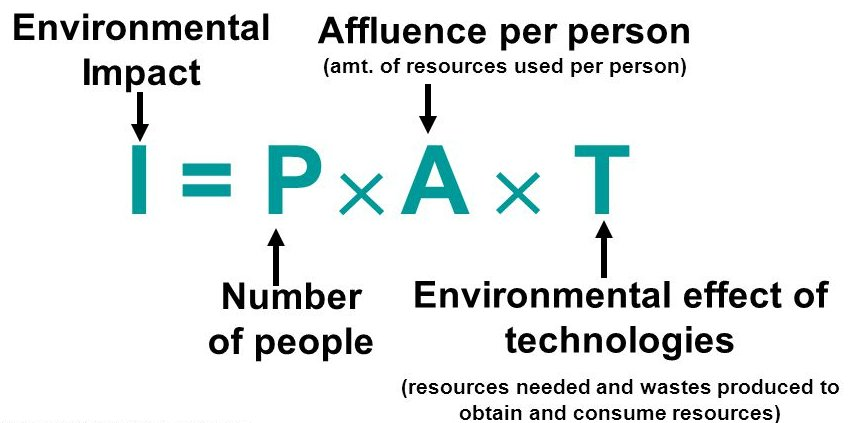
\includegraphics[width=0.7\linewidth]{../images/5-ipat}
		\caption{the I-PAT equation}
		\label{fig:ipat}
	\end{figure}
	
	\ \\
	\textbf{In the last 30 years of the $20^{th}$ century}, population growth was important; affluence growth was important; but the material demand per dollar declined slightly (due to the servitization). \textbf{In the past 20 years}, we have seen a slower population growth, a similar affluence growth, yet an increasing material intensity per dollar (because upper-middle income countries have transitioned through the material intensive phase of industrial development). \textbf{In the future}, population growth will continue, but will become less important in this evolution; affluence will continue growing; and the material demand per dollar will continue to grow, bt not faster, and faster, and faster...
	\\
	\\
	If we look at the reasons behind material demand, we can conclude that the demand will continue to keep growing. This growth will not be equal for all material types. Consider for instance materials needed for the \textbf{energy transition}. Scientists are expecting significantly higher growth rates because of the transition to a carbon neutral energy supply. Lithium for instance, for producing batteries, or for rare earth elements, that we use in magnets for electric vehicles and windmills.
	
	\subsection{Different types of scarcity}
	
	\textbf{Absolute scarcity} is when the amount of raw materials within these reservoirs can only cover the demand for that material for the coming decade or two. There can be a couple reasons for this. First and foremost, the most easily accessible and richest raw materials do deplete. \textbf{The quality of raw materials is often decreasing}. By quality, we understand here the concentration of useful elements they contain. \textbf{Copper} ore, for example, contained 3\% copper at the beginning of the last century; today it contains a good 0.3\%. So, ten times as much copper ore has to be mined for the same amount of copper. Moreover, the new deposits that are found are often difficult to access.
	\\\\
	If we divide the \textbf{current reserve by the current demand}, we see how many years are still left. This is called the \textbf{static depletion index}. However, demand for raw materials changes, for most materials it increases. When we take the \textbf{predicted change in demand into account}, we call this the \textbf{dynamic depletion index}. For a resource with an increase in demand, the dynamic index will be smaller than the static index. An example of this behaviour is the depletion index of Copper (figure \ref{fig:5-static-dynamic-index-copper}).
	
	\begin{figure}[H]
		\centering
		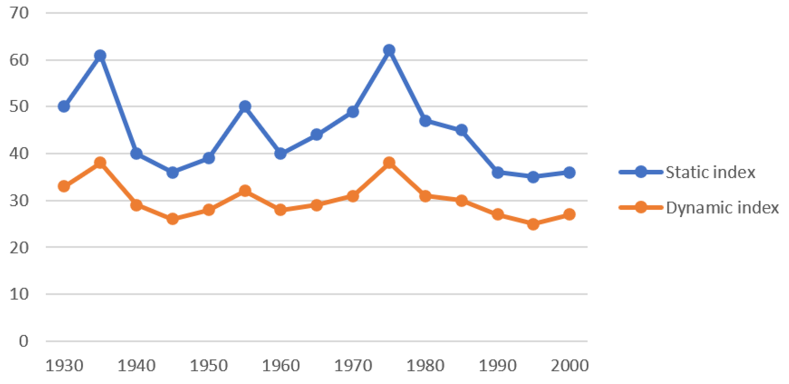
\includegraphics[width=0.7\linewidth]{../images/5-static-dynamic-index-copper}
		\caption{Static and dynamic depletion index of copper}
		\label{fig:5-static-dynamic-index-copper}
	\end{figure}
	
	\ \\
	The \textbf{depletion index remains rather stable}. This can be contributed to the finding of new reserves and the improvement of extraction technology.
	\\\\
	A second aspect of scarcity is that some ores are \textbf{concentrated in only a limited number of countries}. \textbf{Lithium} for example, needed for batteries for electric vehicles, today comes mainly from Bolivia, Chile and Argentina. \textbf{Cobalt} and \textbf{tantalum} are found in Central and South Africa, rare earth metals are mainly mined in China. These ores do not necessarily come from politically stable regions. Regional conflicts can have a major impact on the global price of the raw material. We say such materials are \textbf{economically or geopolitically scarce}. For example, China used an embargo on rare earth exports as an economic threat during the dispute with Japan over the Senkaku Islands in 2010. As a result, the price of some elements, e.g. neodynium,  increased a tenfold in a matter of months.
	\\\\
	Finally, a third scarcity problem is that quite some more exotic elements, often used in high-tech applications, cannot be mined by themselves. They occur in small quantities as a by-product of ores of other metals, called carrier metals. \textbf{Indium}, for example, is found mainly in zinc ore. However, that ore contains three thousand times more zinc than indium. We therefore say that indium is \textbf{structurally scarce}. Two other examples are \textbf{Germanium} (produced from sphalerite, silver, lead, and copper ores) and \textbf{Gallium} (by-product during the processing of bauxite). 
	\newpage
	\subsection{Potential caveats of using bio-based materials}
	
	There are a number of caveats related to the use of bio-based resources. Cultivated or growing \textbf{biomass needs land area}. The land used to grow maize, for example, from which PLA plastic can be made, cannot be used for other crops. A competition may arise between the use of land for materials or for food. Furthermore, soil can become exhausted if used too intensively, and there also will be a impact on biodiversity if new land is cultivated for new crops for materials. 
	\\\\
	Also typical of agriculture is \textbf{the use of fertilisers and pesticides}, which can make the environmental impact of bio-based materials significant.
	\\\\
	Other concerns are about the \textbf{water and energy needed}. Some crops for raw materials, for example cotton, require a lot of water during cultivation. Most crops also require quite a bit of additional energy for tilling the soil, harvesting, and so on. Some new types of bio-based plastics even require more energy and more CO2 emissions to make them than an equivalent conventional petroleum-based plastic. 
	\\\\
	We can conclude that replacing non-renewable materials by bio-based materials is promising, but the impact throughout the entire life cycle has to be carefully investigated.
	
	\subsection{Waste}
	\subsubsection{Amount of waste produced, importance of waste treatment \& Basel Convention}
	
	\textbf{The world generates more than 2 billion tonnes of municipal solid waste annually}. In 2020, an amount of 2.24 billion was estimated. The \textbf{amount of waste production is different in each country} and is mainly related to their income levels. \textbf{Municipal solid waste} includes household, commercial and institutional waste. The composition of such waste is \textbf{very heterogeneous}. 
	\\\\
	The \textbf{two biggest waste streams} when it comes to solid waste are \textbf{electronic waste} and \textbf{plastic waste}.
	\\\\
	Electronic waste contains a \textbf{mix of materials}, including \textbf{toxic substances}, and often \textbf{contains valuable resources}. It is \textbf{one of the fastest-growing waste streams globally}. However, it is not always managed correctly, and often is exported to developing countries where it is managed in uncontrolled and unsafe ways. To address this issue, \textbf{the Basel Convention} was established to \textbf{ensure sound environmental management} of electronic waste and to \textbf{prevent its illegal export} to those countries.
	\\\\
	\textbf{Plastic waste} ends up in \textbf{landfills, is incinerated or is mismanaged}. Nearly 80\% of all \textbf{ocean waste consists of plastics}. Over time, this \textbf{plastic degrades into micro-plastics}. \textbf{The Basel Convention} extended its reach to address plastic waste. This includes a set of actions aimed at preventing and minimizing plastic waste production, and ensuring environmentally sound management practices.
	\\\\
	Considering the huge amount of waste generated worldwide, \textbf{waste minimization and management are key for a more sustainable development}.
	\\\\
	The current trends in waste generation and management have \textbf{significant environmental, social, and economic impacts}. If you think of the more than 2 billion tons of waste produced, over \textbf{30\% of this waste is still not managed} in an environmentally safe manner. This has a lot of negative impacts like a loss of resources, as well as to different environmental and health impacts due to soil and water contamination, and air pollution. For example, \textbf{solid waste is responsible for 3\% of global greenhouse gas emission}. Furthermore, the \textbf{degradation of organic waste} in landfills (and open dumps) \textbf{generates a gas composed mainly of carbon dioxide and methane}. Another example is that \textbf{waste releases hazardous emissions} and particular matter into the air \textbf{when it is burned in an uncontrolled manner}, causing significant health issues. Lastly, \textbf{unmanaged waste degradation} can result in the creation and \textbf{runoff of leachate}, a hazardous liquid that can contaminate water bodies and soil, leading to the contamination of, for example, drinking water, and transmission of diseases.
	\newpage
	
	\subsubsection{Waste hierarchy}
	
	In Europe the European Commission defined the \textbf{waste hierarchy} as a guiding principle for sustainable and integrated waste management. It ranks waste management alternatives based on their potential to minimize environmental impacts, health risks, and promote the recovery of resources. \\
	\\
	At the top of the hierarchy, waste prevention should be prioritized to minimize waste generation. If prevention is not possible, the focus should shift towards promoting the reuse of materials and components. Recycling follows as the next best solution. When none of the above options are feasible, energy recovery from waste is considered. Finally, landfilling represents the least preferable alternative, and waste disposal should be minimized as much as possible. This waste hierarchy is visualized in figure
	
	\begin{figure}[H]
		\centering
		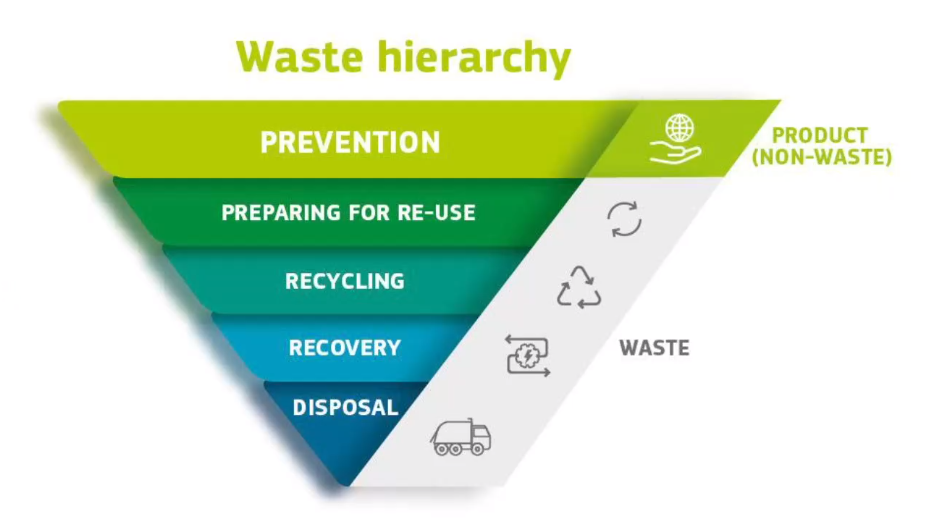
\includegraphics[width=0.7\linewidth]{../images/5-waste-hierarchy}
		\caption{European waste hierarchy}
		\label{fig:5-waste-hierarchy}
	\end{figure}
	
	\ \\
	To conclude, solid waste management is crucial to reduce the negative effects on the environment and human health, and support the transition to a clean and circular economy by promoting resource recovery.  
	\newpage
	
	\subsection{Importance of resource demand in terms of environmental impact}
	
	Figure \ref{fig:5-material-impact} shows \textbf{the share of global impact of different resource types} (biomass, metals, non-metallic minerals and fossil fuels) \textbf{on 4 categories} (climate change, particulate matter health, water stress and land-use related biodiversity loss). 
	\\\\
	When we look at the impact of the four resource types together, we see that they make up \textbf{more than 50\% of the total global greenhouse gas emissions} and \textbf{more than 90\% of biodiversity loss and water stress} with agriculture (biomass) as main driver.
	\\\\
	The \textbf{climate change} impact of metals in mainly due to the \textbf{iron and steel} production and due to \textbf{aluminium} production.
	\\
	\\
	\textbf{Mining} of non-metallic minerals, in particular for sand, can have \textbf{critical impacts on local ecosystems}.
	\\
	\\
	Fossil fuels contribute considerably to \textbf{environmental pollution and especially air pollution}.
	
	\begin{figure}[H]
		\centering
		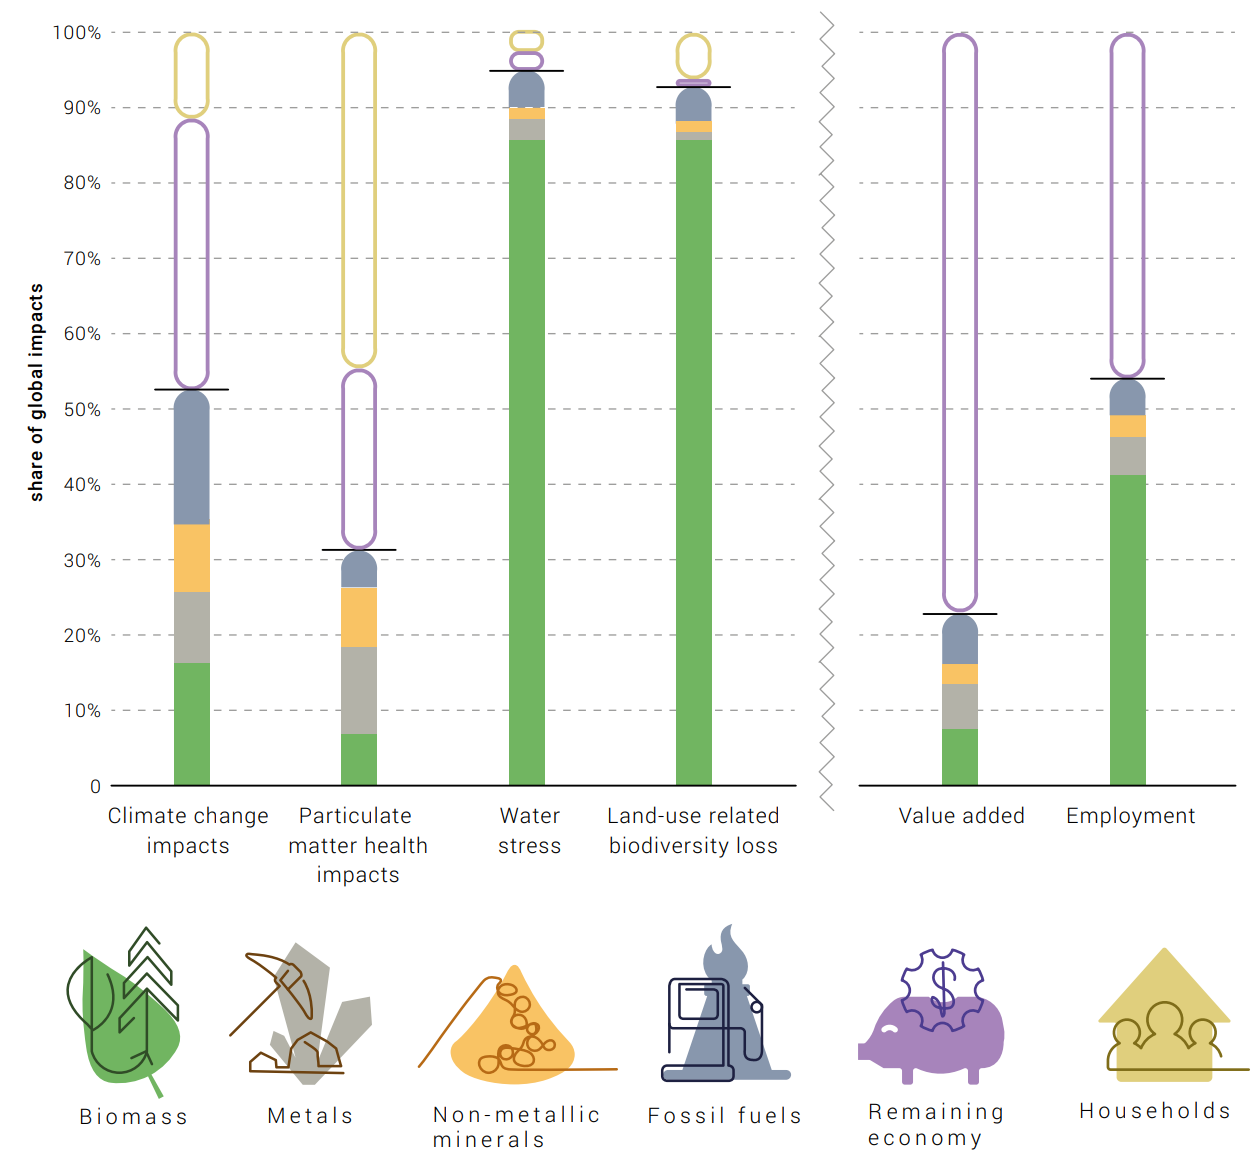
\includegraphics[width=0.9\linewidth]{../images/5-material-impact}
		\caption{Environmental impact of different resource types}
		\label{fig:5-material-impact}
	\end{figure}
	\newpage
	
	\subsection{Reduction of steel and cement productions climate impact}
	
	Cement and steel play a large part in the greenhouse gas emission, and it’s use is still increasing. What are possible ways to reduce these emissions?
	
	\begin{enumerate}
		\item A part of the emissions come from the \textbf{energy used} during production: Decrease production energy by more efficient processes, and use more renewable energy sources for the energy needed during this production processes. 
		\item However, there are also emissions related to the production of the material itself. For example, during the production of cement, a chemical process takes place during which CO2 is released. During steel production, cokes are used in the chemical process to extract iron from iron ore, thereby releasing large amounts of CO2. 
		
		A possible solution is \textbf{using different resources} during these processes. For steel production this is already possible by using hydrogen instead of cokes. However, this requires large investments in new production processes and infrastructure and the production of hydrogen also requires some energy. Another way to reduce the emission of CO2 is by capturing it before it is released into the atmosphere and storing it (Carbon Capture Storage – CCS) or using it elsewhere (Carbon Capture and Utilization – CCU). 
		\item A third solution lies in \textbf{reusing and recycling of waste}, so that the demand for new materials decreases. 
	
	\end{enumerate}
	
	\subsection{Emission, impact category and damage category}
	
	There are three main \textbf{damage categories (end-point indicators)}. Human health, biodiversity and resource depletion. We do not directly affect these categories. These damage categories are indirectly affected through physical and chemical phenomena known as \textbf{impact categories (mid-point indicators)} e.g. climate change. \\
	\\
	We often talk about CO2, an \textbf{emission}, as a cause for climate change, but of course, there are all kinds of other emissions that have similar effects. Think of methane for example. Methane has a much more powerful climate change effect than CO2 by itself. So a kilogram of methane cannot be added to a kilogram of CO2. We will have to take into account its equivalents, its CO2 equivalents. In the case of methane, for example, that's about 23 times more powerful in affecting the climate change effects. 
	
	\begin{figure}[H]
		\centering
		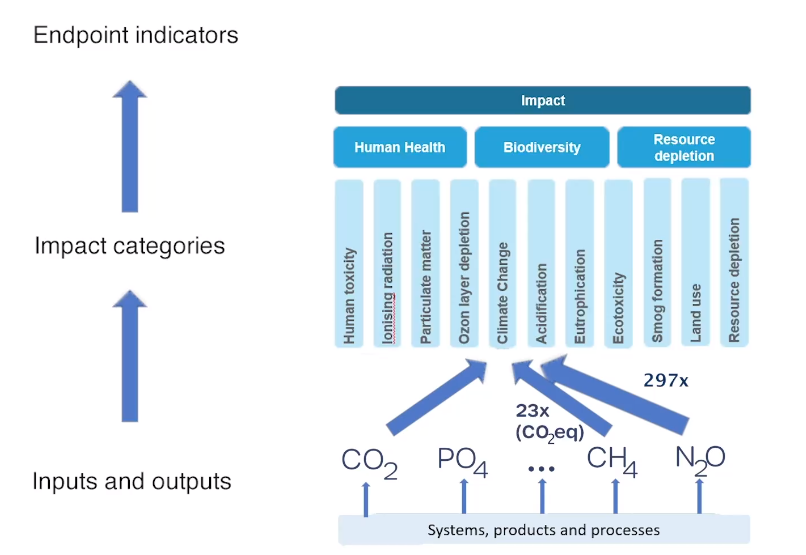
\includegraphics[width=0.7\linewidth]{../images/5-visualisation-for-measuring-impact}
		\caption{Visualisation on how to measure impact (emission $\rightarrow$ mid-point $\rightarrow$ end-point)}
		\label{fig:5-visualisation-for-measuring-impact}
	\end{figure}
	\ \\
	In summary:
	\begin{itemize}
		\item First of all, we will need to quantify the inputs and outputs (emissions) from systems, products and processes
		\item Then, we will learn how to convert those inputs and outputs into impact categories (mid-point categories)
		\item Finally, these impact categories can contribute to damage categories (end-point indicators) of concern, i.e. human health, biodiversity and material depletion
	\end{itemize}
	\ \\
	Fortunately, we have a well-established methodology referred to as \textbf{Life Cycle Assessment} to facilitate this process.
	
	\subsection{Life Cycle Analysis}
	
	Life Cycle Analysis is a tool that allows us to systematically compare alternative design concepts and system designs, based on scientific considerations, when our concern is impact and especially impact avoidance.
	\\\\
	There are four main phases in this procedure. The first one is \textbf{goal and scope definition}, where you need to very clearly determine what is in and what is outside your study. Secondly, once the boundaries are clear, you go for \textbf{inventory}. This can be fairly tedious, sometimes it takes months or even years to collect all the relevant data, but it’s indispensable. We have to get through that data collection stage and only then we can come to the actual \textbf{impact analysis} where we ask ourselves how much these different ins and outs contribute to the different impact categories that we discussed before. The last phase is the \textbf{interpretation}.
	\\\\
	The challenge lies in determining system boundaries, such as what is included or excluded, and defining the \textbf{functional unit}. A functional unit describes a quantity of a product or product system on the basis of the performance it delivers in its end-use application.
	\\\\
	For example:
	\begin{itemize}
		\item When comparing cars, is it normal to compare a two seater to a van that can perhaps contain ten persons, or should you consider five drives by a two seater to have the equivalent functionality as that van?
		\item When comparing paint, are you going to talk about a litre of paint as the functional unit or are you going to talk about the functionality of covering a wall for a certain period? And perhaps with some quality of paint, you may have to repaint it more often or you may have to apply multiple layers to get the same protection level.
	\end{itemize}
	
	
	\subsection{Relative and absolute decoupling}
	
	The concept of decoupling is a strategy put forward by the United Nations, and by the European Commission. The goal is that the need for resources doesn’t follow the growth of economy. Decoupling is not only put forward for resource use, but also for the environmental impact. The UN calls it a dual decoupling: the decoupling of resource use from well-being on the one hand, and impact decoupling decreasing environmental and social impacts per unit of resource use on the other hand.
	\\\\
	When the need for resources is still rising, but at a lower rate than the economy, we have a \textbf{relative decoupling} of resource needs from the economy.
	\\\\
	When the need for resources decreases in absolute terms, while the economy is growing, than we have \textbf{absolute decoupling}.
	
	\begin{figure}[H]
		\centering
		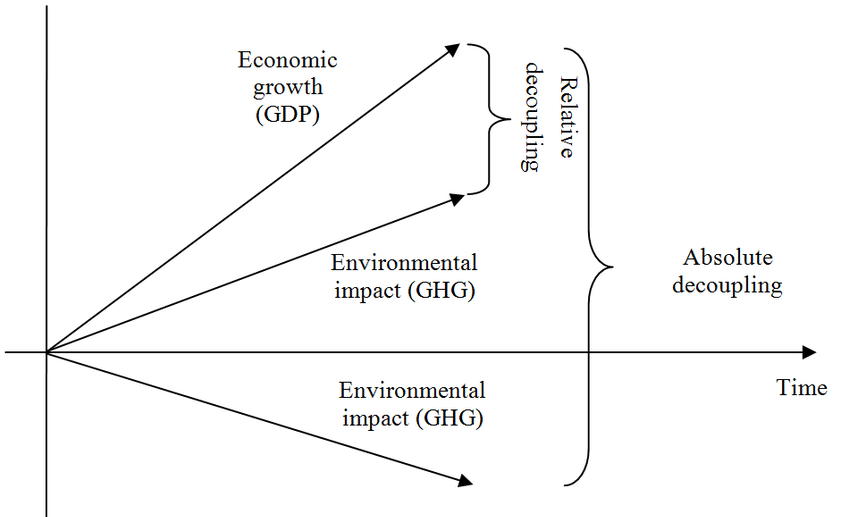
\includegraphics[width=0.6\linewidth]{../images/5-relative-and-absolute-decoupling}
		\caption{Relative and absolute decoupling}
		\label{fig:5-relative-and-absolute-decoupling}
	\end{figure}
	
	\ \\
	If we look at reality, resource use is decoupled from economic growth in Europe. On a global scale however, there is no decoupling at all between resource use and economy, rather on the contrary (figure \ref{fig:5-gdp-dmc-global-eu}). This doesn't mean that Europe is doing better than the rest of the world, it depends for example on how the resource use is measured. Here, we took the classical indicator \textbf{direct materials consumption (DMC)} as measure.
	\\
	\\
	DMC does not take into account the resources used and wasted in other continents for making the products that are imported. \textbf{Only the materials that are physically included in the imported products are accounted for}. Since a lot of basic, resource intensive industry has moved from Europe to other continents, \textbf{part of the decoupling is hence due to this move}. 
	\\
	\\
	Another way of measuring our materials use is by the \textbf{material footprint}, in which all materials consumed in the supply chain to make products, wherever that happened, is included. Typically, the \textbf{material footprint for high income countries is higher than the direct material consumption}, and the decoupling of material footprint from GDP or economic growth is less obvious.
	
	\begin{figure}[H]
		\centering
		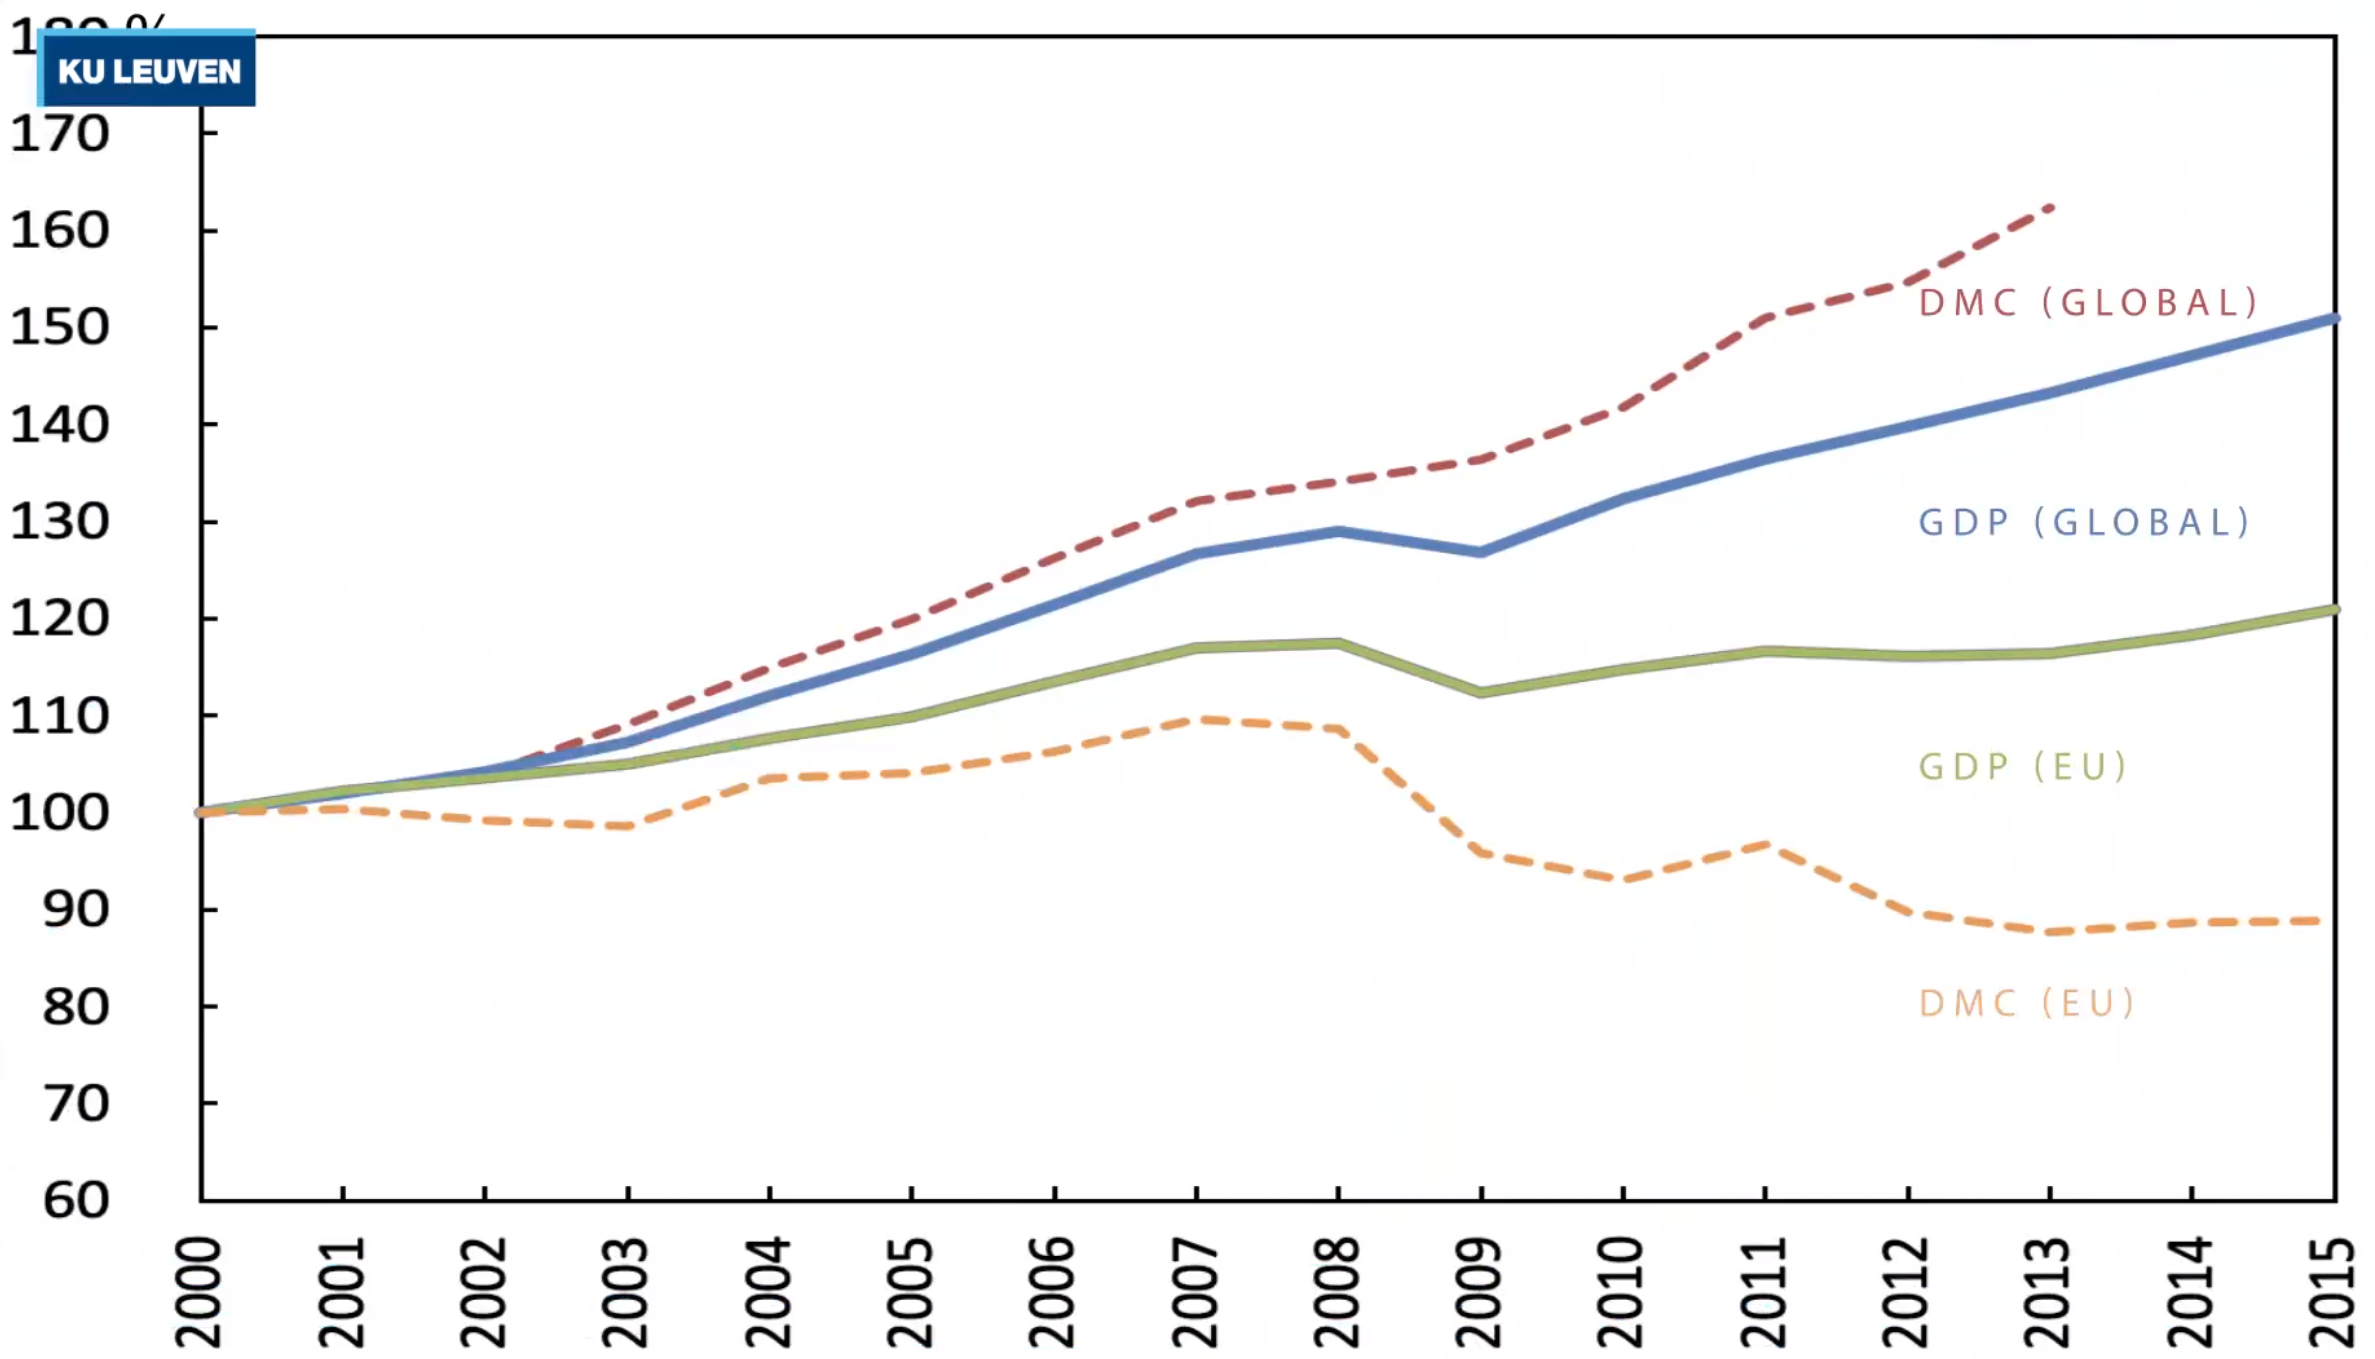
\includegraphics[width=0.8\linewidth]{../images/5-GDP-DMC-GLOBAL-EU}
		\caption{economic growth (GDP) and direct material consumption (DMC)}
		\label{fig:5-gdp-dmc-global-eu}
	\end{figure}
	
	\newpage
	\subsection{Circular economy}
	
	A commonly accepted definition of circular economy says that it is an economy in which the value of materials in the economy is maximised and preserved for as long as possible. This means that the input of new materials and their consumption are minimised, that waste generation is minimised and negative and that environmental impacts are reduced throughout the life cycle of materials. The focus is thus on \textbf{preserving societal value of material goods}.
	\\\\
	This can be done by \textbf{decreasing the number of needed products} by keeping products longer in use, by increasing the lifetime by easier repairing during its life and by reuse. Or products could be used more intensively, by sharing its idle time with other people or by only borrowing the product when you really need it.
	\\\\
	Another way is making the same or similar products with a \textbf{smaller amount of materials}. Strategies to do this are \textbf{ecodesign} of products and \textbf{process intensification} in order to reduce the waste during production. Materials are also saved when \textbf{components from a discarded product still are recovered and remanufactured}.
	\\\\
	Finally, materials and alloys are made out of raw materials. A last question then is whether we can \textbf{reduce the input of new raw materials}, and replace them by \textbf{more sustainable, renewable or recycled raw materials}. 
	\\\\
	\textbf{Recycling} is a cornerstone, but however, \textbf{the last option of the circular economy strategies}. In the circular economy it is even better not to have to discard material, or at least postpone that moment of disposal as much as possible. Preserving value is the main goal.
	\\\\
	To illustrate the difference between a linear and circular economy, consider the example of a shirt:\\
	\\
	\textbf{Linear Economy (Traditional Approach):}
	\begin{itemize}
		\itemsep0em 
		\item Purchase a cotton shirt, contributing to environmentally harmful production.
		\item Discard the shirt when it goes out of fashion.
		\item Eventually, dispose of the shirt, contributing to waste.
	\end{itemize}
	\ \\
	\textbf{Circular Economy Approach:}
	\begin{itemize}
		\itemsep0em 
		\item Purchase a shirt made from locally grown hemp, a more sustainable material.
		\item Borrow shirts for special occasions from a clothing library.
		\item Repair any defects, extending the shirt's lifespan.
		\item Sell, exchange, or donate the shirt at a second-hand shop.
		\item Repurpose the worn-out shirt as a cleaning cloth.
		\item Salvage buttons for reuse.
		\item Finally, send the shirt for textile recycling when no longer usable.
	\end{itemize}
	
\end{document}